\begin{figure}[p]

\begin{center}
\fbox{
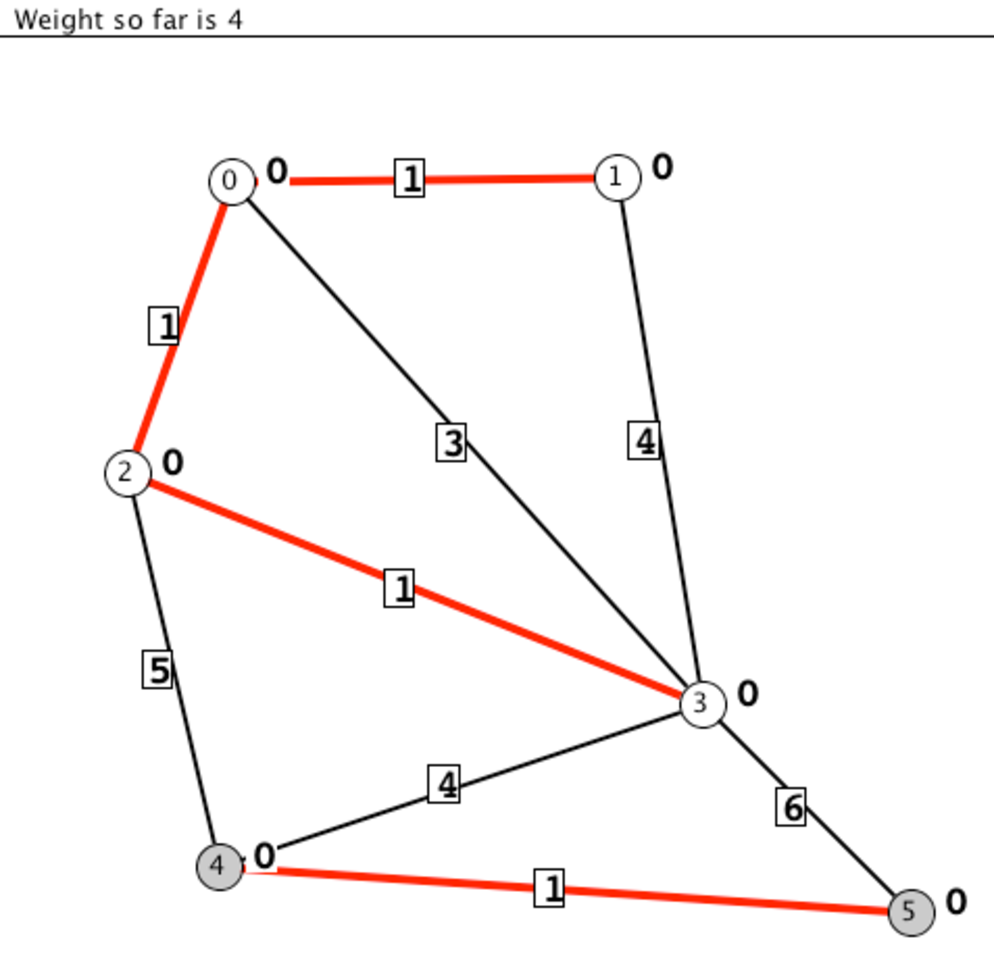
\includegraphics[scale=0.55]{X_kruskal_1}
}

(a) An edge is added to the tree.

\fbox{
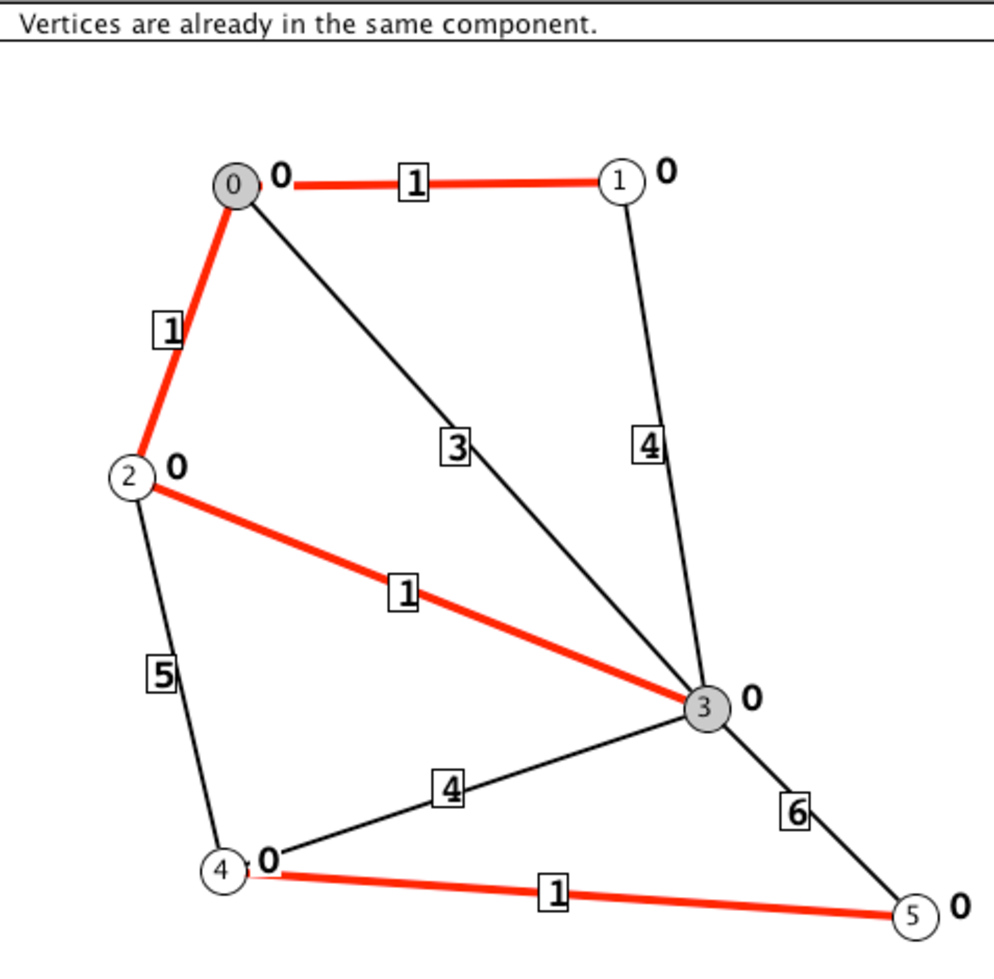
\includegraphics[scale=0.55]{X_kruskal_2}
}

(b) The current edge creates a cycle.

\end{center}

\caption{Two steps in Kruskal's algorithm. A message at the top left of the window describes the state of the algorithm.}

\label{fig:kruskal_pictures}
\end{figure}
